\section{Scenarios, Briefs, Probes}\label{app:scenarios}\label{app:materials}
The supplementary package includes the exact source files for the two scenario stems, the A and B briefs, the condition configs, and the runtime probe constructors. Table~\ref{tab:scenario-materials} summarizes the materials so the allocation and prediction tasks are visible in the PDF.

\begin{table}[h]
\centering\footnotesize
\caption{Synthetic decision materials used in Greenfield and Riverton.}\label{tab:scenario-materials}
\setlength{\tabcolsep}{3pt}\renewcommand{\arraystretch}{1.15}
\begin{tabular}{P{0.10\textwidth}P{0.19\textwidth}P{0.09\textwidth}P{0.27\textwidth}P{0.22\textwidth}}
\toprule
Scenario & Decision setting & Budget & Allocation dimensions & Brief contrast \\
\midrule
Greenfield & Community Investment Committee & \$10M grant & Education, Healthcare, Green Spaces, Infrastructure, Economic Development & Education-oriented community data versus wellbeing, green-space, and mental-health data \\
Riverton & AI Transition Committee at a manufacturing and technology firm & \$5M transition budget & Automation, Workforce Training, Employee Support, Innovation Lab, Data Infrastructure & Efficiency and technology-infrastructure data versus workforce readiness and employee-support data \\
\bottomrule
\end{tabular}
\end{table}

\paragraph{Runtime allocation probe.} The runtime probe asks each agent to distribute 100 percentage points across the five scenario-specific areas. It requires one area per line in the form \texttt{Area: [number]\%} and asks for no commentary. This stricter probe is the one used for all allocation-vector scoring.

\paragraph{Runtime prediction probe.} The post-discussion prediction probe asks each agent to predict how a named target agent would distribute 100 percentage points across the same five areas. It uses the same one-line-per-area format and asks for no commentary. Prediction MAE is computed from these predicted vectors against the target agent's realized post-discussion allocation.

\paragraph{Off-topic transfer probes.} The BFI-10 probe follows the original short inventory and the PsychoBench LLM adaptation~\citep{Rammstedt2007_BFI10,PsychoBench}. The prompt asks for ten integer Likert ratings from 1 to 5 only, with no explanation. The conformity probe uses paired natural and majority-pressure responses over 15 items inspired by classic Asch-style conformity framing~\citep{Asch1956_Conformity}, with randomized order between phases. The consistency probe asks the same final-position question in three phrasings and scores average pairwise word overlap, following a lightweight CogMir-inspired probe design~\citep{CogMir}. These operational definitions take precedence over informal ``personality'' or ``agreement'' labels.

\section{Statistics, Calibration, and Provenance}\label{app:stats}\label{app:audit}

\begin{table}[h]
\centering\footnotesize
\caption{Scoring formulas for the five SocCogEval instruments.}\label{tab:metrics}
\setlength{\tabcolsep}{4pt}\renewcommand{\arraystretch}{1.15}
\resizebox{\textwidth}{!}{%
\begin{tabular}{llll}
\toprule
Instrument & Per-agent score $y_i$ & Range and direction & Test against contrast \\
\midrule
Allocation divergence & $|x_{i,j}^{A}-x_{i,j}^{B}|$ per dim $j$ & higher \(=\) more divergent & per-dim CI excludes 0, majority rule \\
Prediction MAE & $\mathrm{MAE}(\hat{x}_{i\to j}, x_j)$ & lower \(=\) better at modeling $j$ & Wilcoxon paired (in $<$ out) \\
BFI-10 L1 drift & $\sum_{f}|s_{i,f}^{\text{post}}-s_{i,f}^{\text{pre}}|$ & higher \(=\) more drift, 0 to 20 & run-level exact permutation \\
Conformity rate & $\#\{\text{switched to majority}\}/\#\text{eligible}$ & 0 to 1 & two-sample on per-agent $y_i$ \\
Consistency score & agreement across 3 phrasings & 0 to 1, higher \(=\) more consistent & two-sample on per-agent $y_i$ \\
\bottomrule
\end{tabular}}
\end{table}

\textbf{Original agent-level estimator.} The submitted analysis computed allocation divergence, BFI L1 drift, conformity rate, and consistency score per agent ($n{=}\text{reps}\times 8$ agent-observations per condition), and prediction MAE per (predictor, target) pair aggregated per predictor. CIs came from a two-level cluster bootstrap that resamples replicas with replacement and then agents within each sampled replica (10{,}000 resamples), with Welch's $t$ as the parametric reference. Table~\ref{tab:decomp-agent} keeps those values. The main text leads with the run-level exact tests in Table~\ref{tab:decomp}, whose point estimates are identical because every run has eight agents.

\begin{table}[h]
\centering\footnotesize
\setlength{\tabcolsep}{3.5pt}
\caption{BFI-10 decomposition with the original agent-stratified bootstrap and Welch $p$.}\label{tab:decomp-agent}
\resizebox{\textwidth}{!}{%
\begin{tabular}{ll ccc ccc}
\toprule
& & \multicolumn{3}{c}{Greenfield} & \multicolumn{3}{c}{Riverton} \\
\cmidrule(lr){3-5}\cmidrule(lr){6-8}
Contrast & Isolates & $\bar\Delta$ ($g$) & 95\% CI & $p$ & $\bar\Delta$ ($g$) & 95\% CI & $p$ \\
\midrule
\tableinput{tables/app_decomp_agent.tex}
\bottomrule
\end{tabular}}
\end{table}

\begin{table}[h]
\centering\footnotesize
\caption{Primary and solo-control BFI-10 run means, ordered by replica index.}\label{tab:runvalues}
\begin{tabular}{llP{0.64\linewidth}}
\toprule
Scenario & Condition & Run means \\
\midrule
\tableinput{tables/run_rows.tex}
\bottomrule
\end{tabular}
\end{table}

\begin{table}[h]
\centering\footnotesize
\caption{Dependence diagnostics on agent BFI L1 scores, with $\mathrm{DE}=1+7\max(0,\widehat{\mathrm{ICC}})$.}\label{tab:icc}
\begin{tabular}{llrrrr}
\toprule
Scenario & Condition & ICC(1) & DE & Nominal $n$ & Effective $n$ \\
\midrule
\tableinput{tables/icc_rows.tex}
\bottomrule
\end{tabular}
\end{table}

\textbf{Calibration.} Repeated SRM extractions on two pilot dialogues recover the same fields in all repeated runs, with 5 extractions per dialogue and a target of at least 90\%. Condition $C_4$ produces detectable allocation shifts on 2 of 5 dimensions in Greenfield and 4 of 5 dimensions in Riverton, leaving room for interaction effects to appear on top. Under $T{=}0.0$, $C_5$ produces zero allocation divergence on at least 3 of 5 dimensions in both scenarios. A temperature sweep confirms that increasing $T$ inflates the $C_5$ floor monotonically, supporting $T{=}0.0$ for deterministic instruments (Figure~\ref{F5}).

\begin{figure}[h]
\centering
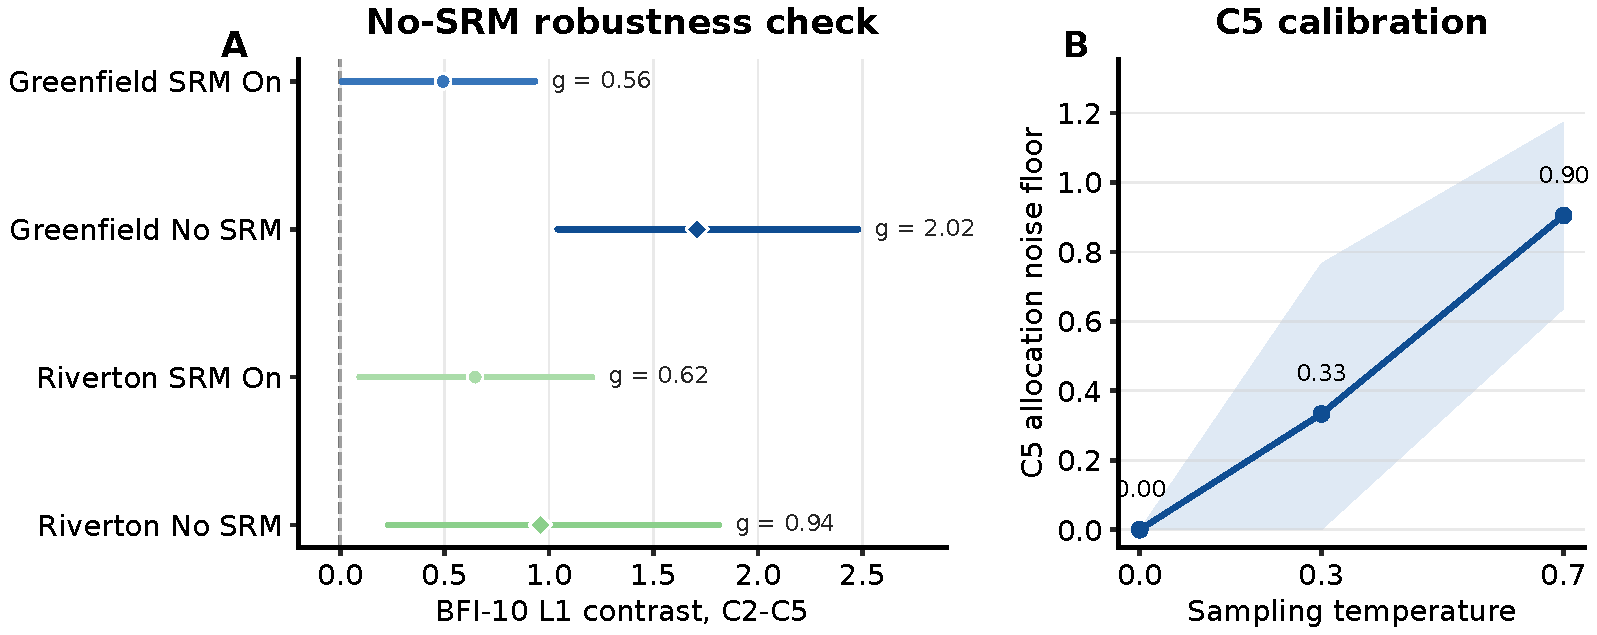
\includegraphics[width=0.92\textwidth]{figures/A2.pdf}
\caption{No-SRM robustness (left) and the $C_5$ calibration floor across temperature (right).}\label{F5}
\end{figure}

\textbf{Instrument-specific floor.} At BFI temperature 0.7, all three $C_5$ raw-response payloads and score payloads differ in each scenario. Agent pre/post score equality is 0.042 in Greenfield and 0.208 in Riverton. At allocation temperature zero, all three nominal $C_5$ runs have identical raw responses and allocation arrays, and every agent's allocation is unchanged pre/post. Repeating this deterministic payload contributes no new floor variation, which is why the $C_5$-dependent contrasts are qualified in Section~\ref{sec:exp-limits}.

\textbf{Provenance.} The release identifies every selected run and retains its configuration, pre/post measurements, and summary. The original 128-run ledger comprises 56 primary runs, 60 historical cross-variant $C_2/C_5$ runs, and 12 no-SRM runs. Thirty added cross-variant $C_4$ runs and ten formal $C_6$ runs bring the total to 168. Frozen-state temperature-zero probes reuse existing trajectories and do not increase the independent run count. The primary and $C_6$ intervals use 50,000 bootstrap draws with fixed seeds, and the other run-level intervals use the same estimator. For historical runs, exact request tokens, immutable provider revisions, tokenizer revisions, precision, batch placement, and run-time source commits are incompletely recorded. Source reconstruction establishes matching initial prompt construction for a corresponding named agent in $C_2$ and $C_4$. The post-treatment requests intentionally differ through stored interaction memory, and probes leave agent state unchanged in the current implementation.

\subsection{Compute and Reproduction}\label{app:cost}
Total wall-clock time on primary Qwen3-122B-FP8 (TP=2, both scenarios, 56 production runs, excluding the no-SRM robustness check) is approximately 90 GPU-hours on H200. The completed no-SRM check adds approximately 38 wall-clock hours on the same TP=2 server (about 76 additional H200 GPU-hours). Cross-architecture API runs incur single-digit dollar API fees. The local visual variant on Qwen3-VL-32B takes approximately 5 GPU-hours per scenario. These historical estimates do not cover the added $C_4$ runs, temperature re-probing, or $C_6$, whose audited call and token totals are in the artifact tables. The compact measurement package supports offline numerical verification without an LLM service. It includes selected run configurations, raw pre/post responses, derived scores, summaries, selection manifests, and hashes. Live regeneration additionally requires model weights or provider access and a recorded serving configuration.

\section{Matched Non-Social Control}\label{app:c6}
The $C_6$ design was frozen on 25 July 2026. Operational clarifications and a throughput amendment were recorded before formal outcomes were inspected. Each round has three generation stages and one extraction stage, with a barrier between stages. Each generation stage submits one independent call for every agent. Each agent sees its own current-round outputs, and previous rounds are accessed through the same memory interface as the interaction protocol. The first prompt asks for private reasoning about the allocation problem, values, evidence, and tradeoffs. The second asks the agent to reconsider that reasoning from another angle and resolve a tension or uncertainty. The third asks for its current best allocation reasoning and any change in its own view. All three prohibit addressing, quoting, predicting, or simulating another person.

Formal $C_6$ runs used tensor parallelism 1, maximum context length 8,192, FP8, eager execution, GPU memory utilization 0.92, and at most eight concurrent sequences. Two incomplete serial Greenfield attempts were operationally aborted and excluded, and all ten formal runs restarted under the amended serving schedule. Every audited formal run has 720 content calls and 240 extraction calls. $C_6$ records request and output hashes, serving metadata, and token counts. Historical $C_2$ did not save equivalent token usage, so we claim neither realized token equality nor a token-normalized social effect.

\subsection{Belief-Probe Time Course}\label{app:timecourse}
Belief probes run every five rounds and leave conversation history and memory unchanged. Their free text rarely states all five allocation shares (14\% of probes), so we track wording instead. For each run and probe round, \emph{wording separation} is the mean Jaccard word overlap between agents in the same group minus the mean overlap between agents in different groups, after removing stop words. Groups are agents 0--3 and 4--7, as in every other group-level analysis. Figure~\ref{fig:timecourse} uses the ledger-selected primary $C_1$, $C_2$, and $C_3$ runs and the ten $C_6$ runs, with run-bootstrap bands.

\begin{figure}[h]
\centering
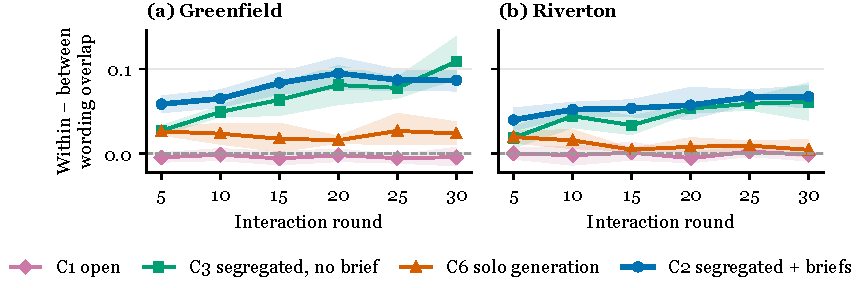
\includegraphics[width=\textwidth]{figures/time_course.pdf}
\caption{Within-group minus between-group wording overlap of belief probes over rounds.}\label{fig:timecourse}
\end{figure}

Within-group convergence grows over the episode in the two segregated interaction conditions. On Greenfield, separation moves from $+0.059$ to $+0.087$ in $C_2$ and from $+0.027$ to $+0.109$ in $C_3$ between rounds 5 and 30, and on Riverton from $+0.040$ to $+0.067$ and from $+0.019$ to $+0.061$. The solo-generation condition starts near the $C_3$ level because of its asymmetric briefs and then stays flat or declines ($+0.026$ to $+0.024$, and $+0.020$ to $+0.004$). The open-network $C_1$ stays at zero. Agents in segregated conditions talk only within their group, so part of this convergence is shared vocabulary from the conversations themselves. The measure is descriptive and is computed from stored probe text after the experiments.

\section{Cross-Variant Tables and Routing}\label{app:cross}\label{app:routing}

\begin{table}[h]
\centering\footnotesize
\setlength{\tabcolsep}{3.5pt}
\caption{BFI-10 L1 drift, $(C_2){-}(C_5)$, across model variants (original agent-level estimator).}\label{tab:cross}
\begin{tabular}{l ccc ccc c}
\toprule
& \multicolumn{3}{c}{Greenfield} & \multicolumn{3}{c}{Riverton} & Same dir \\
\cmidrule(lr){2-4}\cmidrule(lr){5-7}
Variant & $\bar{\Delta}$ & $g$ & $p$ & $\bar{\Delta}$ & $g$ & $p$ & GF, RV \\
\midrule
\tableinput{tables/app_cross_c2c5.tex}
\bottomrule
\multicolumn{8}{l}{\footnotesize $^{\dagger}$Raw $\bar{\Delta}$ is load-bearing. $g$ is inflated because the small-$n$ pooled SD on its $C_5$ approaches the floor.} \\
\end{tabular}
\end{table}

\begin{table}[h]
\centering\footnotesize
\caption{Additional variants, run-level $(C_2){-}(C_4)$, three runs per condition and scenario.}\label{tab:cross-c4}
\begin{tabular}{lrrr}
\toprule
Variant & Greenfield & Riverton & Scenario average \\
\midrule
\tableinput{tables/cross_rows.tex}
\bottomrule
\end{tabular}
\end{table}

The cross-variant analogue of Table~\ref{tab:cross} is provided for conformity and consistency per scenario per variant in the released analysis files. Conformity replication is mixed, with Gemini-2.5-Flash significant on Greenfield, GPT-4.1-mini significant on Riverton, and others mostly null. Consistency replication is broad, with 5 of 6 variants positive on Riverton and 3 of 6 on Greenfield, with no significant decrease anywhere. These $(C_2){-}(C_5)$ estimands are not pooled with the $(C_2){-}(C_4)$ panel.

Each additional-variant $C_2/C_4$ scenario cell contains three completed runs. Selection uses the last complete timestamped retry for each prescribed cell, as specified by the original cross-variant analysis, and all complete candidates remain listed. A completed cell with a reversed effect remains included. For DeepSeek-V3, historical $C_2$ configurations record \texttt{deepseek-chat}, while the selected $C_4$ runs record \texttt{deepseek-v4-flash}. Historical immutable revisions are not available, so we report the identifier difference without treating it as a verified same-revision experiment. Endpoint configuration used DeepSeek-V3, GPT-4.1-mini, Gemini-2.5-Flash, and Llama-4-Scout via provider APIs, with Llama-4-Scout routed through OpenRouter. The primary analysis filters cross-variant replicas out of the within-Qwen3-122B-FP8 factorial via run-id pattern. The sign summary averages the two scenario differences within each variant before counting directions, so ten scenario cells are not treated as ten independent models.

\section{Signed and Temperature Robustness}\label{app:signed}

\begin{table}[h]
\centering\footnotesize
\caption{Signed factor diagnostics $\kappa_f$, $C_2-C_4$, with run-bootstrap intervals (10,000 draws).}\label{tab:signed}
\begin{tabular}{llrrc}
\toprule
Scenario & Factor & $\kappa_f$ & 95\% interval & Agreement \\
\midrule
\tableinput{tables/signed_rows.tex}
\bottomrule
\end{tabular}
\end{table}

The deterministic re-probe uses the same ten BFI items and reverse-coding rules, replacing only probe temperature. Saved post-treatment states retain their history, so it is a sensitivity analysis over the same experimental trajectories rather than an independently generated replication. Factor analyses are descriptive and are not corrected for multiple comparisons, for example by false-discovery-rate control~\citep{Benjamini1995}. Figure~\ref{fig:app-part2-breakdown} gives the factor-level drift and the secondary Part 2 metrics from the original analysis.

\begin{figure}[h]
\centering
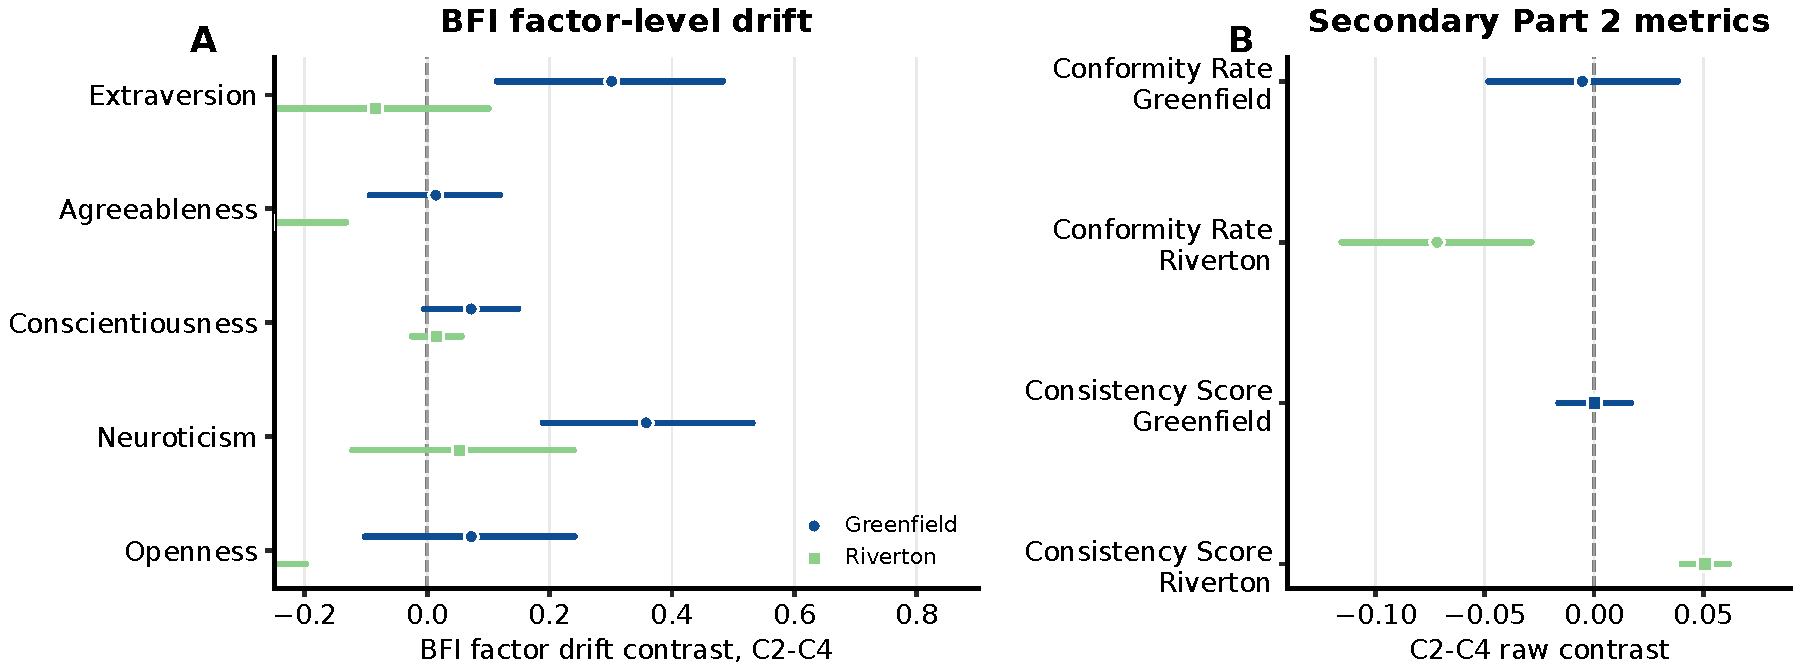
\includegraphics[width=0.92\textwidth]{figures/A3.pdf}
\caption{Part 2 breakdown: BFI-10 factor-level drift (left) and secondary metrics (right).}\label{fig:app-part2-breakdown}
\end{figure}

\section{Supporting Analyses}\label{app:secondary}

\begin{table}[h]
\centering\footnotesize
\caption{Verbatim-history no-SRM check, original agent-level estimator (3 vs.\ 3 replicas).}\label{tab:nosrm}
\resizebox{\textwidth}{!}{%
\begin{tabular}{lcccc}
\toprule
Scenario & $C_2$ mean & $C_5$ mean & $\bar{\Delta}$ ($g$) & 95\% CI, $p$ \\
\midrule
\tableinput{tables/app_nosrm_agent.tex}
\bottomrule
\end{tabular}}
\end{table}

No-SRM $C_2$ run means are $[2.000,2.250,3.188]$ in Greenfield and $[1.500,2.500,1.563]$ in Riverton, against $C_5$ means $[0.938,0.688,0.688]$ and $[1.125,1.063,0.500]$. Exact two-sided tests enumerate $\binom{6}{3}=20$ allocations and give $p=0.10$ in both cases, so the agent-level Welch values in Table~\ref{tab:nosrm} are not used as confirmatory evidence.

\begin{table}[h]
\centering\footnotesize
\begin{minipage}[t]{0.47\textwidth}\centering
\caption{Secondary $C_2-C_4$ summaries.}\label{tab:secondary}
\resizebox{\linewidth}{!}{%
\begin{tabular}{llrr}
\toprule
Scen. & Instrument & Diff. & 95\% CI \\
\midrule
\tableinput{tables/secondary_rows.tex}
\bottomrule
\end{tabular}}
\end{minipage}\hfill
\begin{minipage}[t]{0.5\textwidth}\centering
\caption{Per-dimension $C_2-C_4$ allocation (pp).}\label{tab:allocation}
\resizebox{\linewidth}{!}{%
\begin{tabular}{llrr}
\toprule
Scen. & Dimension & Diff. & 95\% CI \\
\midrule
\tableinput{tables/allocation_rows.tex}
\bottomrule
\end{tabular}}
\end{minipage}
\end{table}

\section{Extended Related Work}\label{app:related}
\textbf{Social influence before LLMs.} Repeated averaging of neighbors' opinions leads groups to consensus~\citep{DeGroot1974}, and later models keep a weight on each person's initial position while peers pull opinions together~\citep{Friedkin1990}. Experiments separate informational influence, where others count as evidence, from normative pressure to agree~\citep{Deutsch1955,Asch1956_Conformity}. Communication can also remove the diversity that makes independent judgments useful in aggregate~\citep{Lorenz2011}, and small committed minorities can tip a population's convention~\citep{Centola2018}. Similar convention dynamics appear in LLM populations~\citep{FlintAshery2025_Conventions}. Our segregated $C_2$ groups are a controlled version of this setting, with the off-topic BFI-10 probe asking whether influence extends past the discussed question.

\textbf{LLM agents as a study population.} Machine behavior has been proposed as an empirical science of individual and collective agent behavior~\citep{Rahwan2019}. Language models are used to simulate survey respondents and human-subject studies~\citep{Argyle2023,Aher2023_SimulateHumans}, generative agent-based models couple agent decisions with later interactions~\citep{Ghaffarzadegan2024}, and LLM simulations are argued to be a promising research method~\citep{Anthis2025_SocialSim}. Other work cautions that synthetic responses can misrepresent variation and mislead inference~\citep{Bisbee2024}, raises validity and reproducibility questions for generative social science~\citep{Bail2024}, and separates model responses from human participants~\citep{Dillion2023}. Treating each agent as one role a model plays~\citep{Shanahan2023} fits our reading of BFI-10 scores as response profiles. Close to our question, initially undifferentiated LLM agents develop distinct personalities through communication~\citep{Takata2024}. Our design adds a brief held fixed, matched no-interaction and solo-generation controls, and a transfer endpoint unrelated to the conversation.

\textbf{Measuring LLM personality.} Cognitive-psychology batteries characterize model behavior~\citep{Binz2023,CogBench}. Prompted personas can express target traits~\citep{Jiang2024_PersonaLLM}, and LLM-specific test sets aim at reliable and valid trait measurement~\citep{Lee2025_TRAIT}. Evidence on reliability is mixed. Some scales are consistent under tested conditions~\citep{Huang2024_ScaleReliability}, while other studies find unreliable answers, sensitivity to option order and prompt wording, and self-reports that do not predict behavior~\citep{Shu2024_PsychReliability,Gupta2024_SelfAssessment,Han2025_PersonalityIllusion,Sclar2024_PromptFormat}. Familiar inventories may also be contaminated~\citep{Han2026_Contamination}. We use BFI-10 as a fixed probe and compare its change across matched conditions, so a constant bias in the instrument cancels in the contrast. We do not claim that the inventory measures an LLM's personality.

\textbf{Influence and agreement in multi-agent LLM systems.} Debate can improve factuality and reasoning~\citep{Du2024_MultiagentDebate} and encourage divergent thinking~\citep{Liang2024_DivergentDebate}, and debating evaluators change each other's judgments~\citep{Chan2024_ChatEval}. Models agree with users and peers~\citep{Sharma2024_Sycophancy,Cheng2025_ELEPHANT}, defer to agents presented as authorities~\citep{Choi2026_Authority}, and conform to a majority~\citep{Weng2025_Conformity}. Interacting LLMs revise funding allocations in ways shaped by past opinions~\citep{CisnerosVelarde2025_Funding}. Multi-agent failures are often coordination and verification errors~\citep{Cemri2025_MASFailures}, and reliability drops over long conversations~\citep{Laban2025_LostMultiTurn}. These studies measure behavior inside the interaction. SocCogEval measures what the interaction leaves behind on an unrelated probe, and the solo-generation control separates partner effects from extended generation.

\textbf{Inference with dependent units.} When one unit's treatment affects another's outcome, causal estimands must be defined over exposure structures~\citep{Hudgens2008,Aronow2017}. Our estimand is defined at the run level, where the whole group receives the interaction treatment. Treating observations within one unit as replicates is pseudoreplication~\citep{Hurlbert1984}, cluster-robust inference is fragile with few clusters~\citep{Cameron2015}, and evaluation items that share a source need clustered errors~\citep{Miller2024_ErrorBars}. With 3 to 8 runs per cell, we use exact permutation over all allocations~\citep{Phipson2010}, run-bootstrap intervals~\citep{Efron1979}, and Hedges' bias-corrected $g$~\citep{Hedges1981} as a secondary scale.
